% ===========================================
% Electrical Schematics
% Written by: Braidan Duffy
%
% Date: 07/18/2022
% Last Revision: 07/26/2022
% ============================================

\setchapterstyle{koa}
\chapter{Electrical Schematics}
\setchapterpreamble[u]{\margintoc}
\labch{electrical_schemcatics}

One of the key pieces of instrumentation design is the electrical schematic and Printed Circuit Board (PCB).

\section{Schematic Basics}
\todo{Set chapter image to a schematic OR paste a big image of a goo schematic somewhere on this page}
The electrical schematic is a key piece of documentation that communicates to engineers what the circuit is comprised of and how it will work.
All modern electronic devices have schematics of varying complexity and depth that describe how electrons flow from one piece to another and document what behaviors can be expected during operations.
To understand these documents is to understand how a product fundamentally works, and to understand how to make these documents well is a skill that needs to practiced and refined by reviewing schematics and having yours reviewed.
For now, we will go over the basics and give you a fundamental understanding of what the schematic entails and what most of the symbols you might encounter mean.
\section{Basic Notation}


\section{Component Symbols}
The core of the schematic are the 2D representations of the components in the design called, \emph{symbols}. 
There are a variety of symbols that all mean different things and can have slightly different meanings depending on the drawer and application.
The symbols covered henceforth are the standard-accepted versions so they should be what you see in most schematics you may encounter or be asked to work with or design.

    \subsection{Power Symbols} 
    Power symbols are the set of symbols that indicate where the electrical power is coming from, and where it is going.

        \subsubsection*{The Power Source Rail} 
        the power source rail is typically denoted by a vertical "T" or arrow as shown below, and can be labelled with 3V3,\sidenote{Sometimes, it is easier to use a letter to represent a decimal point. 
        In this case, 3V3 is 3.3 volts.}
        5V, VBAT, VBUS, or any other source name.

        \begin{figure}[h!]
            \labfig{power_rail_symbol}
            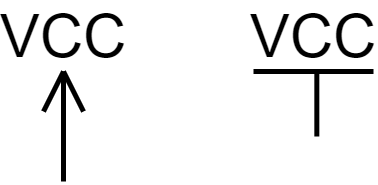
\includegraphics[height=1in]{electrical_schematics/power_rail_symbols.png}
            \caption[Power Rail Symbols]{Schematic symbols for power rails.
            The value label at the top can be any value like 3V3, 5V, etc.}
        \end{figure}

        \subsubsection*{The Power Sink Rail} 
        The power sink rail is the "ground" path from electrical energy will flow back to the negative terminal of the power supply. 
        It is typically represented by a vertical "$\perp$" or upside down tree as shown in \hl{FIGURE}.
        It should always be labelled "GND" with sometimes a prefix of "A" or "D" to denote a different analog or digital ground reference.

        \begin{figure}[h!]
            \labfig{power_sink_symbol}
            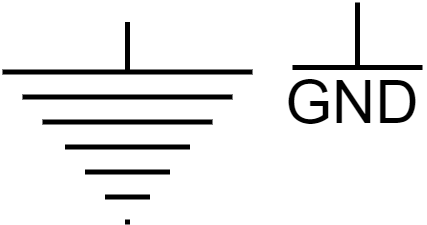
\includegraphics[height=1.25in]{electrical_schematics/ground_rail_symbols.png}
            \caption[Power Rail Symbols]{Schematic symbols for ground rails.}
        \end{figure}

        \subsubsection*{Power Supplies} are generally represented by a circle with a positive and negative input.
        In order to differentiate a DC supply and AC supply, we can use either a plus/minus or sine wave, respectively.
        Both of these symbols are represented in the figure below.

        \begin{figure}[h!]
            \labfig{power_source_symbol}
            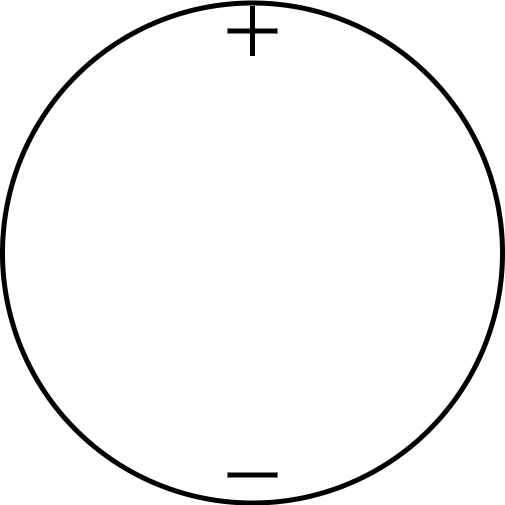
\includegraphics[height=1in]{electrical_schematics/DC_source_symbol.png}
            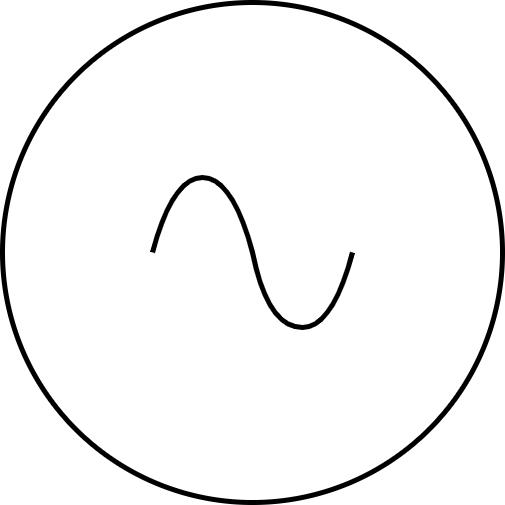
\includegraphics[height=1in]{electrical_schematics/AC_source_symbol.png}
            \caption[Source Symbols]{Schematic symbols for DC and AC power sources, respectively. 
            Notice how the AC power source uses a sinusoidal wave to differentiate it.}
        \end{figure}

        \paragraph*{The Battery} is a subset of DC power supply for embedded applications or circuits that will not have access to a general DC power supply.
        These components are meant to store a large amount of electrical charge for a long duration and be able to discharge it into a circuit to run it.
        Some batteries, like Lithium Ion batteries, are capable of being recharged using special integrated circuits and power supplies.
        Others, like alkaline batteries, are only usable once and must be disposed of properly when they are depleted.

    \begin{marginfigure}[-2in]
        \labfig{battery_real}
        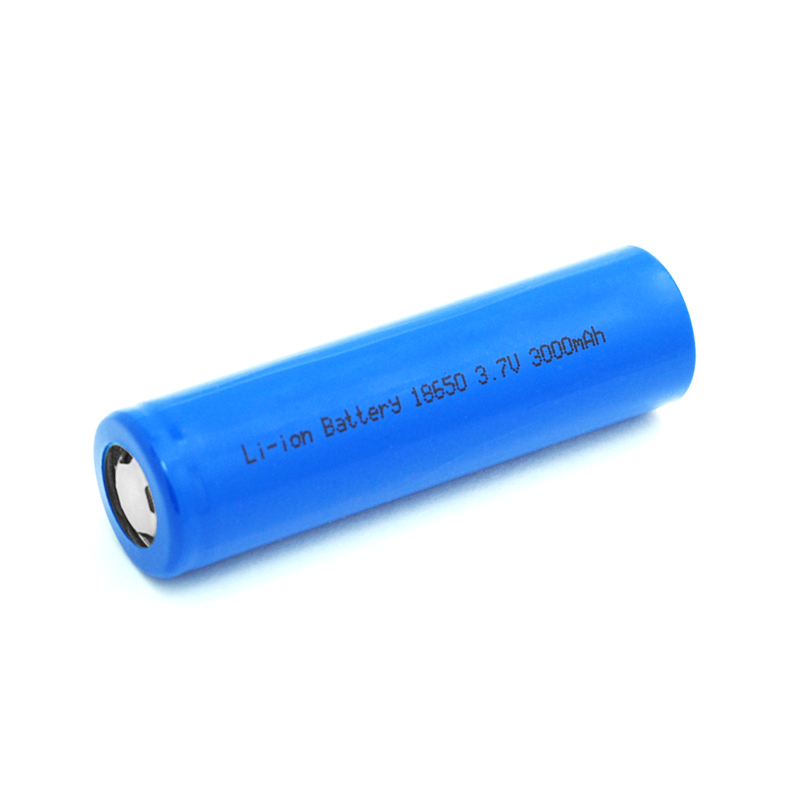
\includegraphics[]{electrical_schematics/battery.jpg}
        \caption[Chip Resistors]{18650 Li-ion battery. 
        Retrieved from \href{https://himaxelectronics.com/product-item/18650-3000mah-li-ion-battery-cell/}{Himax Electronics}}
    \end{marginfigure}

    \begin{figure}[h!]
        \labfig{battery_symbol}
        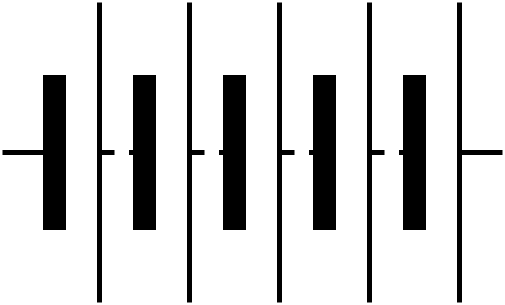
\includegraphics[height=1in]{electrical_schematics/battery_symbol.png}
        \caption[Resistor Symbols]{Schematic symbol for a battery. 
        The different sized lines that comprise the battery symbol represent the different plates that are within modern battery construction.}
    \end{figure}

    \subsection{Basic Components} 
    The following basic component symbols represent discreet components within an electrical circuit.
    Most of these components perform a single service within the circuit and must be used in conjunction with other basic parts to achieve an action.

        \subsubsection*{Resistors} 
        Resistors are components that resist the flow of current and can be used to dissipate energy, reduce voltage levels, or limit current going into other components.
        There are represented with a jagged line or box with "whiskers" as shown in the figure below.

        \begin{marginfigure}[-1in]
            \labfig{resistor_real}
            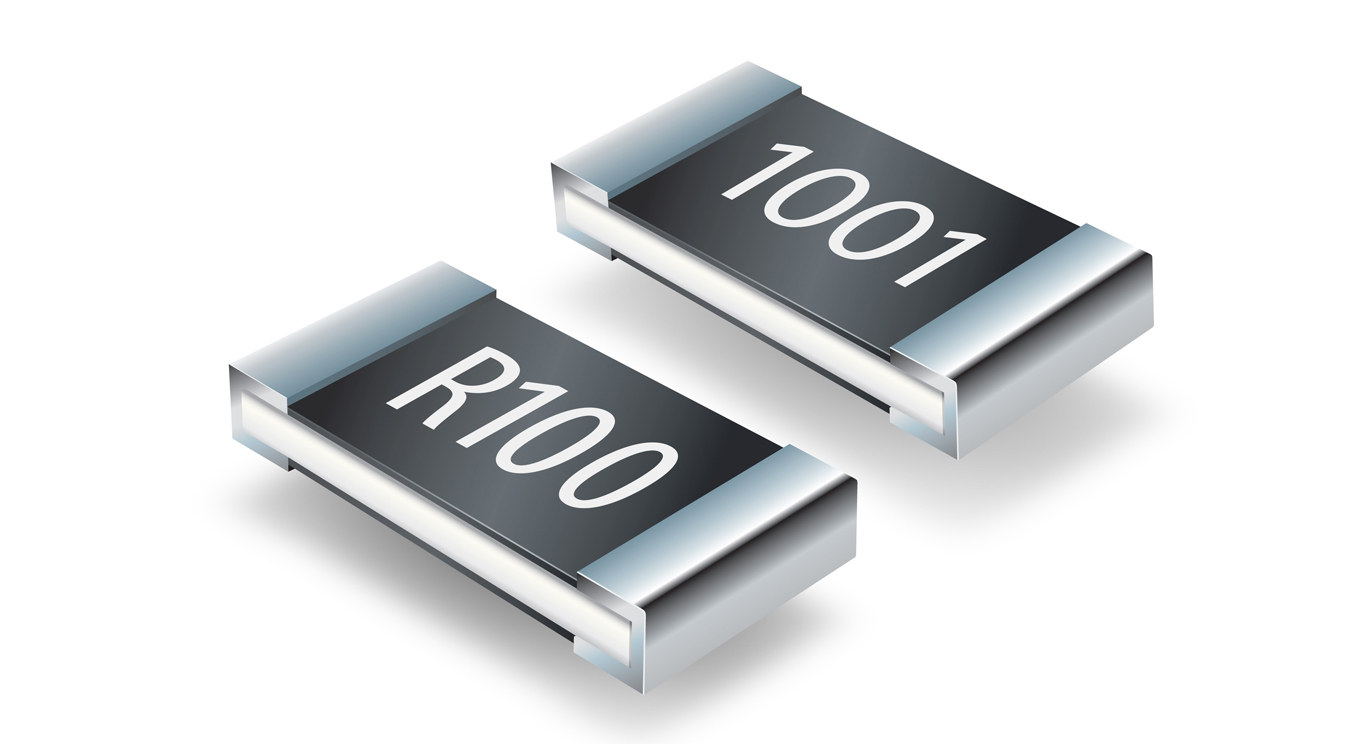
\includegraphics[]{electrical_schematics/chip_resistors.jpg}
            \caption[Chip Resistors]{Surface mount chip resistors. 
            Retrieved from \href{https://www.mpdigest.com/2018/01/24/thick-film-chip-resistors/}{MPDigest}}
        \end{marginfigure}

        \begin{figure}[h!]
            \labfig{resistor_symbol}
            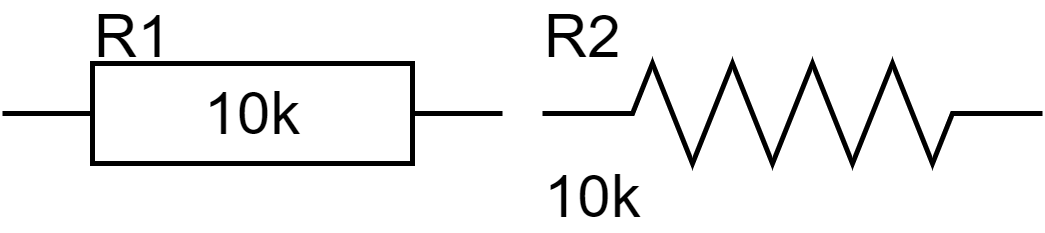
\includegraphics[width=4in]{electrical_schematics/resistors_symbols.png}
            \caption[Resistor Symbols]{Schematic symbols of resistors. 
            European standard is the left, US standard to the right.}
        \end{figure}

        \paragraph*{The Potentiometer} is a variable resistor that changes resistance depending on the position of "wiper" across a band of resistive material.
        Typically, these components are turned by human operators and can be used as an input to determine a variety of things, depending on application.

        \begin{marginfigure}[-1in]
            \labfig{potentiometer_real}
            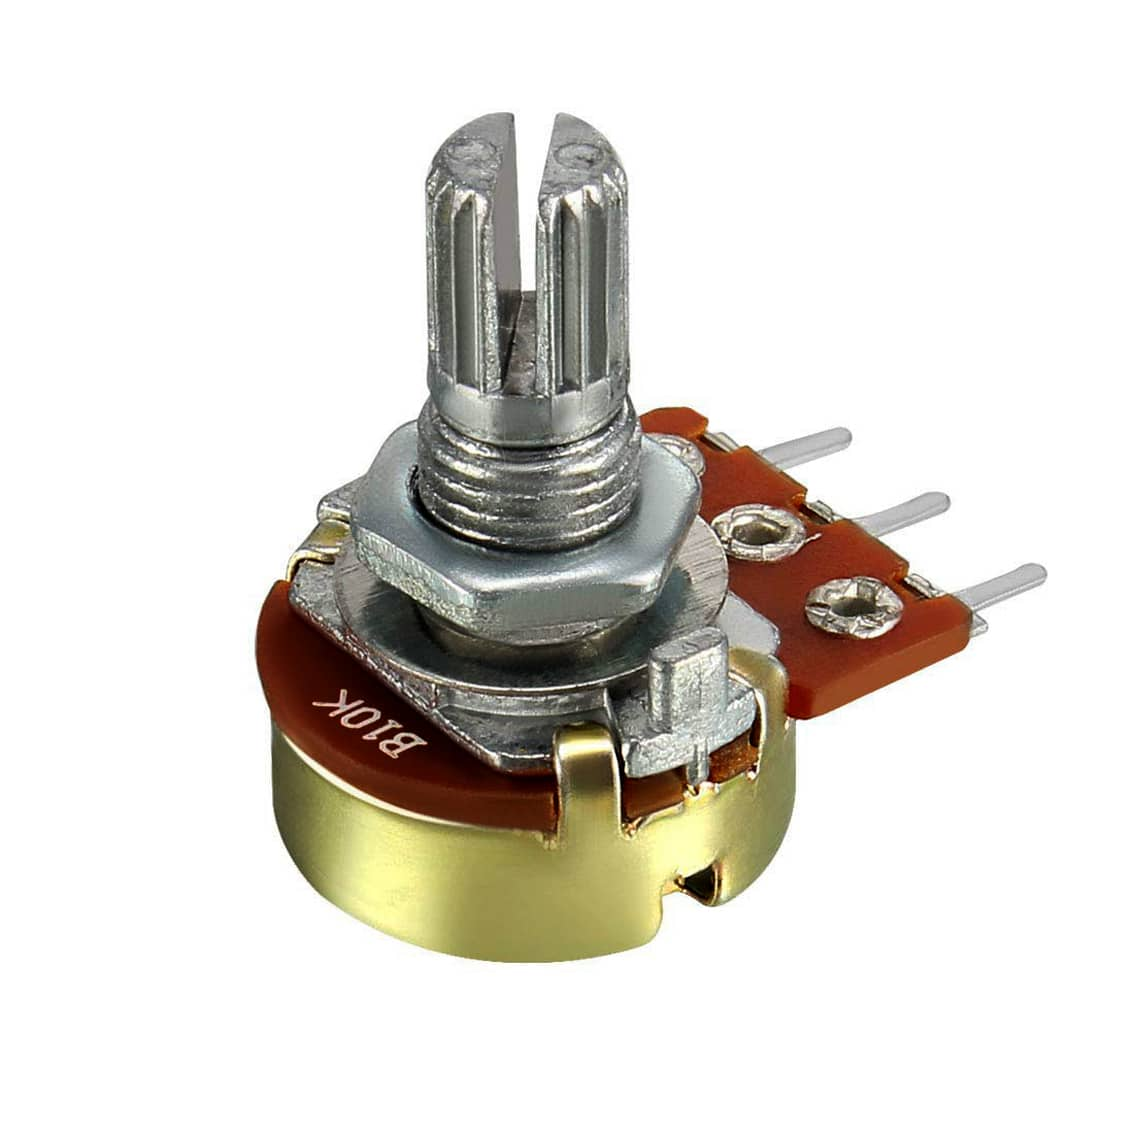
\includegraphics[height=1.5in]{electrical_schematics/potentiometer.jpg}
            \caption{Panel mount potentiometer.
            Retrieved from \href{https://www.phippselectronics.com/product/10k-potentiometer-panel-mount-breadboard-friendly-pack-of-2/}{Phipps Electronics}}
        \end{marginfigure}

        \begin{figure}[h!]
            \labfig{potentiometer_symbol}
            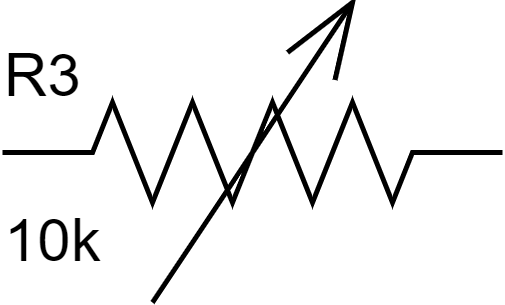
\includegraphics[height=1.5in]{electrical_schematics/potentiometer_symbol.png}
            \caption[Potentiometer Symbol]{Schematic symbols for potentiometers. Notice the arrow through the resistor to demark it from standard resistors. The value at the bottom is the maximum resistance.}
        \end{figure}

        \paragraph*{Photoresistor}
        The photoresistor is a variable resistor that changes resistance depending on the intensity of light interacting with it
        Typically, these components are used as basic light sensors that can be used for presence detection, sun tracking, or other light intensity measurement.

        \begin{marginfigure}[-1in]
            \labfig{photoresistor_real}
            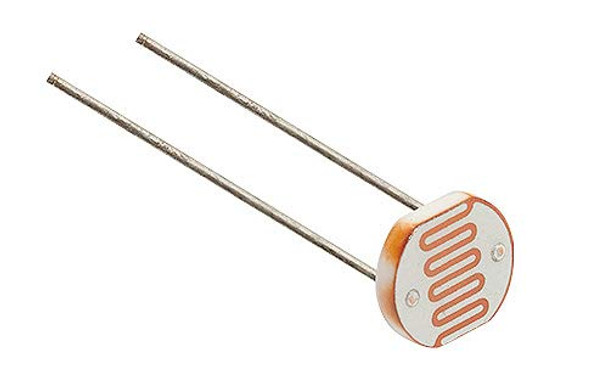
\includegraphics[]{electrical_schematics/photoresistor.jpg}
            \caption{LDR photoresistor.
            Retrieved from \href{https://www.pixelelectric.com/sensors/light-sound/light-color-sensor/5528-ldr-mini-photoresistor/}{Pixel Electric}}
        \end{marginfigure}

        \begin{figure}[h!]
            \labfig{potentiometer_symbol}
            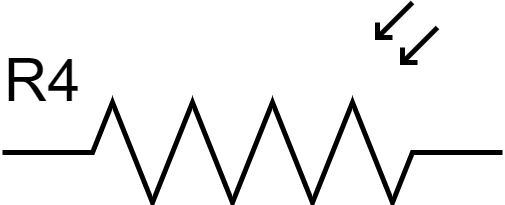
\includegraphics[height=1in]{electrical_schematics/photoresistor_symbol.png}
            \caption[Potentiometer Symbol]{Schematic symbols for photoresistors. The arrows pointed towards the resistor indicate its light dependency.}
        \end{figure}

        \subsubsection*{Capacitors}
        Capacitors are components that store and discharge electrical energy.
        They use parallel conducting plates isolated from each other with a dielectric that allows charges to build up on one face at a certain voltage, then discharge when at a lower voltage.
        This gives capacitors the ability to smooth ripples in voltage levels (called a decoupling).
        This is commonly used to decouple components from electrical noise upstream of their power supply, giving them a cleaner electrical input.
        Additionally, they can provide a high current energy source that has some advantages over traditional batteries.
        In most circuits, you will encounter ceramic capacitors (pictured to the side) that do not hold a log of charge, but work for most applications.
        These capacitors are bi-directional or non-polarized so they can be placed in any orientation on the schematic.

        \begin{marginfigure}[-2in]
            \labfig{capacitors_real}
            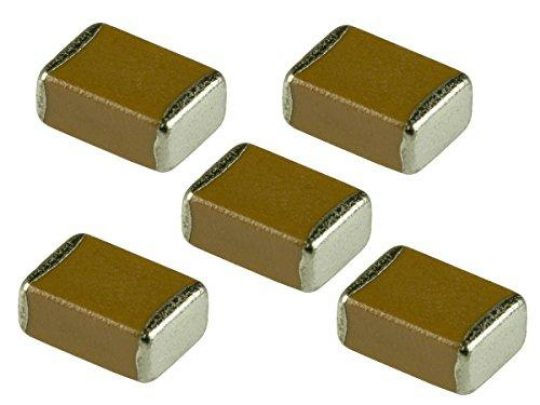
\includegraphics[]{electrical_schematics/capacitors.jpg}
            \caption{Chip ceramic capacitors.
            Retrieved from \href{https://universal-solder.ca/product/320-pcs-ultimate-smd-1206-ceramic-capacitors-kit-10pf-to-22uf/}{Universal Solder}}
        \end{marginfigure}

        \begin{figure}[h!]
            \labfig{capacitors_symbols}
            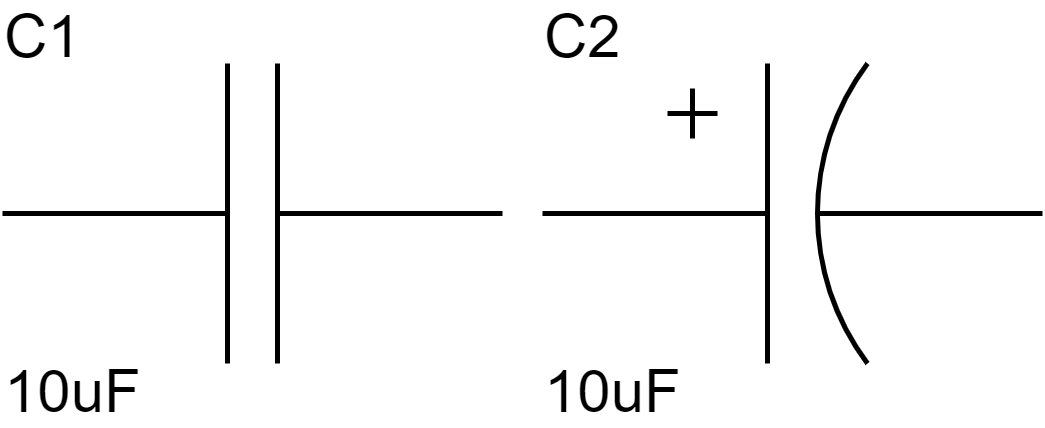
\includegraphics[height=1.5in]{electrical_schematics/capacitor_symbols.png}
            \caption[Potentiometer Symbol]{Schematic symbols for Capacitors. 
            On the left is the symbol for a non-polarized bi-directional capacitor.
            On the right is the symbol for an electrolytic or polarized capacitor.}
        \end{figure}

        \paragraph*{Electrolytic Capacitors} are polarized or uni-directional capacitors that use a liquid electrolyte compared to the ceramic ones used in non-polarized capacitors.
        These capacitors must be placed in a specific orientation otherwise they may become damaged and could explode!
        On electrical schematics, the negative terminal of these capacitors is denoted by a curved line, like shown above.
        Even though, you must closely pay attention to how the capacitor is orientated, the electrolytic capacitor provides a much high energy density compared to the ceramic capacitors, making them more suited for high power application.

        \begin{marginfigure}[-1.5in]
            \labfig{electro_capacitor}
            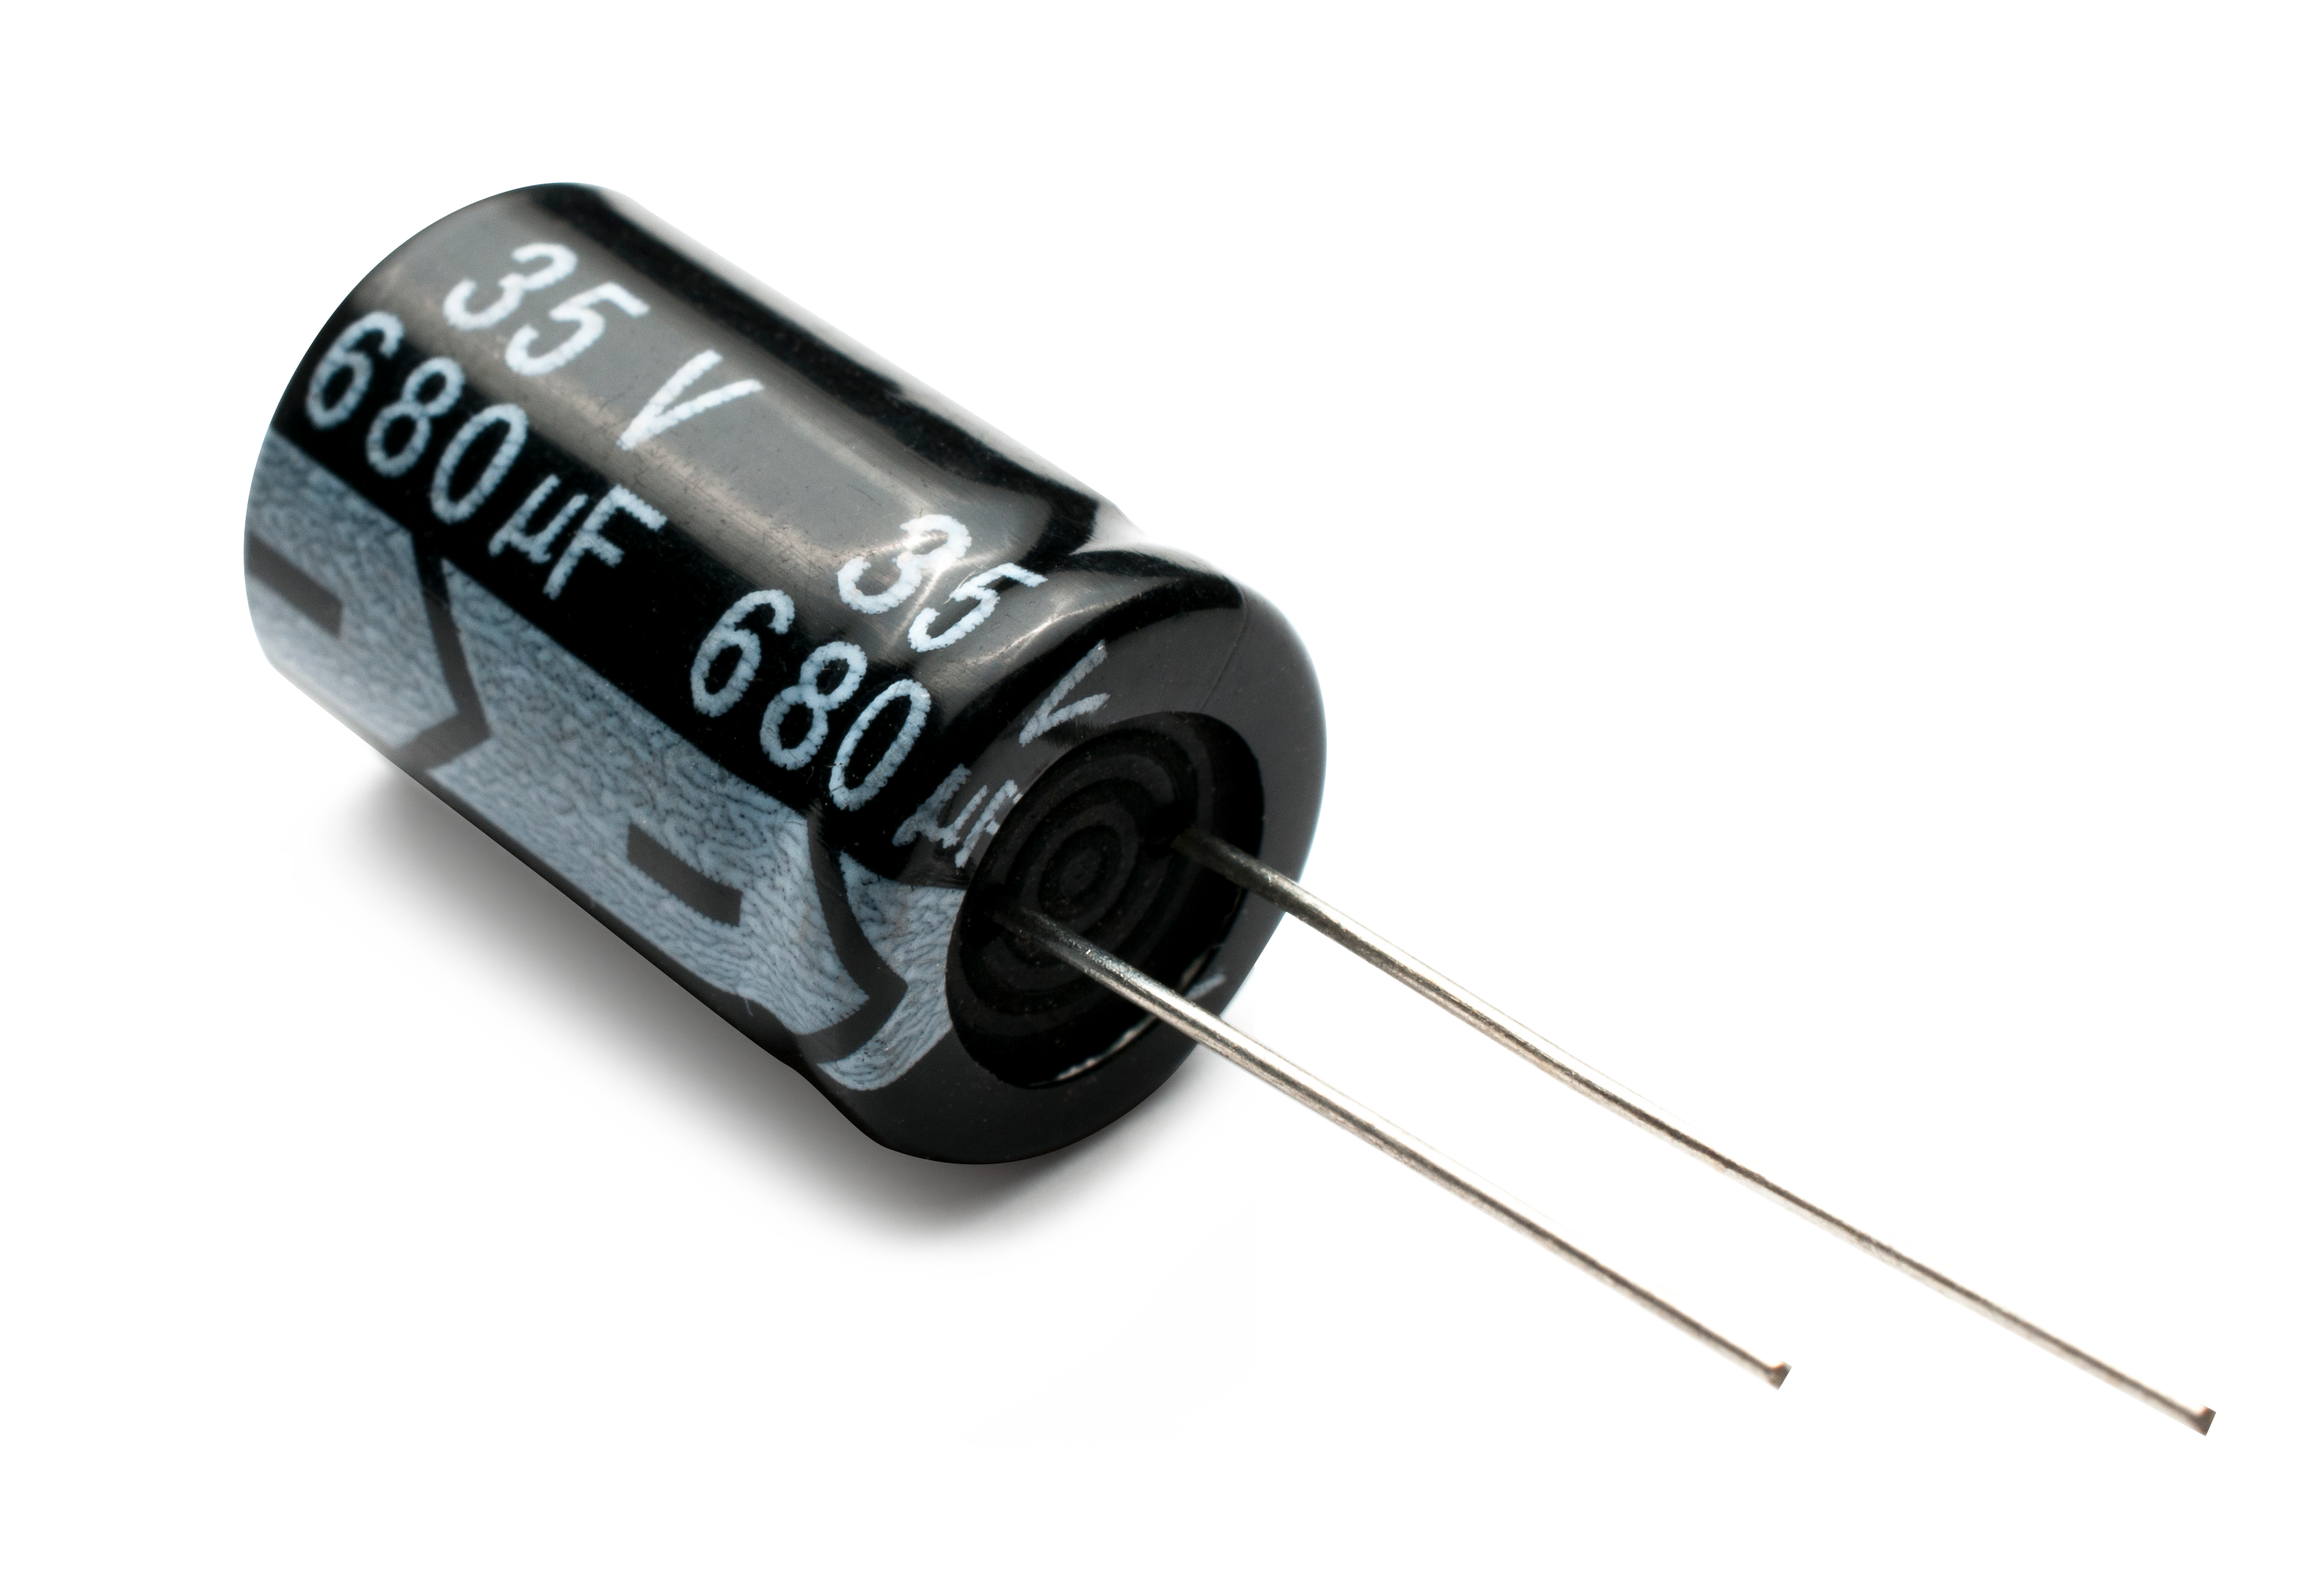
\includegraphics[]{electrical_schematics/electro_capacitor.png}
            \caption{Electrolytic capacitor.
            Notice the longer lead indicates the positive terminal and the negative terminal is clearly marked with a stripe on the casing.
            Retrieved from \href{https://www.srgllc.com/us/en/settlements/electronics/electrolytic-capacitors-indirect-purchaser}{SRG LLC}}
        \end{marginfigure}

        \subsubsection*{Inductors}
        Inductors are tiny electromagnetic that wind conducting wire around an iron or air core.
        When alternating electrical current is passed through the inductor, some of the energy is buffered in the magnetic field of the electromagnet. 
        You can think of them as electrical flywheels that store moving charge and can discharge it to maintain a more constant "flow".
        This makes inductors useful for resisting changes in current or acting as the analogue to capacitors in AC circuits.

        % \begin{marginfigure}[-1in]
        %     \labfig{inductor_real}
        %     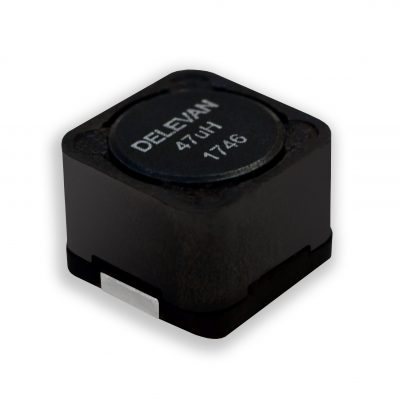
\includegraphics[]{electrical_schematics/inductor.jpeg}
        %     \caption{Surface mount inductor.
        %     Retrieved from \href{https://www.ept.ca/products/shielded-surface-mount-power-inductors-deliver-high-reliability/}{EP\&T}}
        % \end{marginfigure}

        \begin{figure}[h!]
            \labfig{inductor_symbol}
            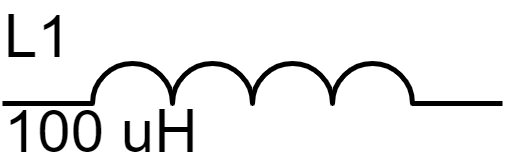
\includegraphics[height=1in]{electrical_schematics/inductor_symbol.png}
            \caption[Inductor Symbol]{Schematic symbol for inductors.}
        \end{figure}

        \subsubsection*{Diodes}
        Diodes are used to restrict current flow in a certain direction.
        This is accomplished using some electrochemical wizardry and comes at the cost of a little bit of voltage drop through the diode.
        But, the main property of the diode makes it invaluable for protecting circuits against reverse polarity, dissipating AC current, or even rectifying AC voltages into DC.

        \begin{marginfigure}[-1in]
            \labfig{diode_real}
            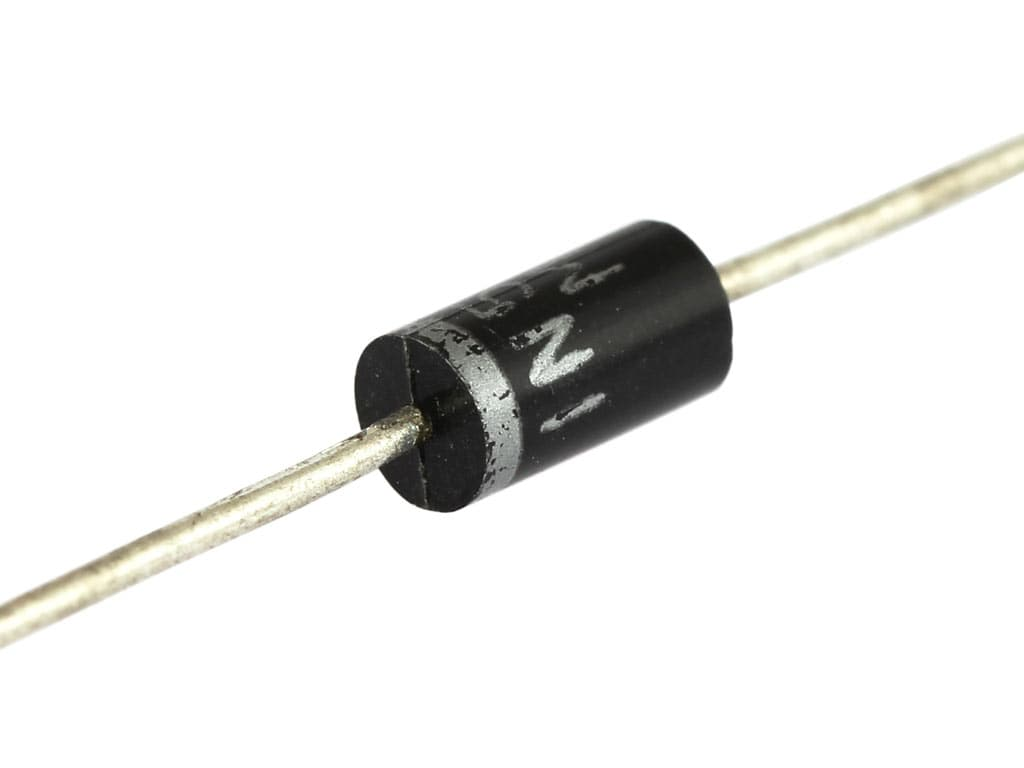
\includegraphics[]{electrical_schematics/diode.jpg}
            \caption{Through hole diode as commonly found in Arduino kits.
            Retrieved from \href{https://analyseameter.com/2016/03/diodes-types-operation-symbol-applications.html}{AnalyzeAMeter}}
        \end{marginfigure}

        \begin{figure}[h!]
            \labfig{diode_symbol}
            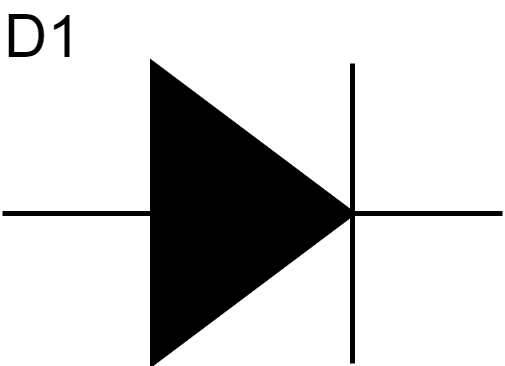
\includegraphics[height=1in]{electrical_schematics/diode_symbol.png}
            \caption[Diode Symbol]{Schematic symbol for diodes.}
        \end{figure}

        \paragraph*{Light Emitting Diodes (LEDs)} are diodes that siphon a little bit of electrical energy to emit photons at specific wavelengths.
        These components are ubiquitous in any application that requires a simple human interface such as light indicators, RGB gaming products, or flashlights.
        LEDs are smaller, easily scaled to almost any production scale, and more energy efficient compared to most other light sources in use today.

        \begin{figure}[h!]
            \labfig{led_symbol}
            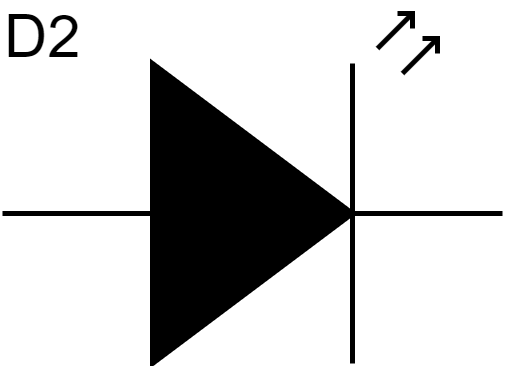
\includegraphics[height=1in]{electrical_schematics/led_symbol.png}
            \caption[LED Symbol]{Schematic symbol for light emitting diodes.}
        \end{figure}

        \paragraph*{Zener Diode} are special diodes that restricts the current flow direction up to a certain breakdown voltage.
        When that voltage is achieved, current is allowed to flow against the diode, without damaging it, making it useful in applications like circuit protection.

        \begin{figure}[h!]
            \labfig{zener_diode_symbol}
            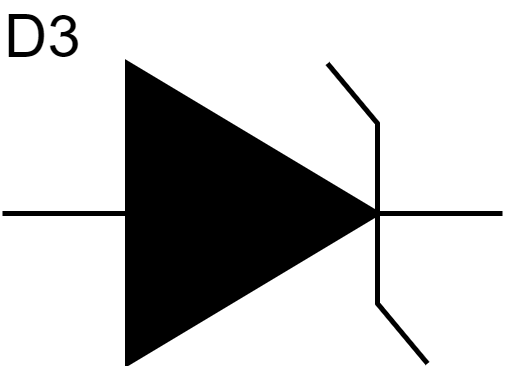
\includegraphics[height=1in]{electrical_schematics/zdiode_symbol.png}
            \caption[Zener Diode Symbol]{Schematic symbol for Zener diodes.}
        \end{figure}

        \paragraph*{Schottky Diode} are other special diodes that have a very low voltage drop across it, making it ideal for applications where flow restriction is necessary, but power loss needs to be considered.
        These are commonly used to control the flow of charge within a battery pack of multiple cells.
        As these cells discharge, they can have slightly different voltages, meaning some energy loss will occur as one battery tried to equalize voltage with another in the pack.
        Schottky diodes ensure the charges flow only from the batteries to the draw outside the pack, without wasting much energy.

        \begin{figure}[h!]
            \labfig{schottky_diode_symbol}
            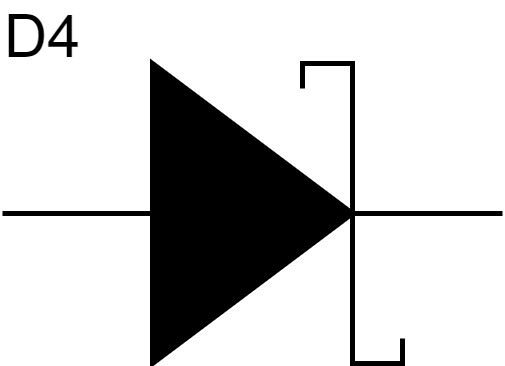
\includegraphics[height=1in]{electrical_schematics/schdiode_symbol.png}
            \caption[Schottky Diode Symbol]{Schematic symbol for Schottky diodes.}
        \end{figure}

        \subsubsection*{Crystal Oscillators}
        Oscillators resonate at a certain frequency depending on the type of crystal used and the coupling capacitors matched to it.
        These driving most modern computational circuits as they generate a very clean DC square wave. 
        Some components use the rising or falling edge of this wave to trigger register shifts, calculations, anything else needed to perform its duty.
        Therefore, for any circuit that requires a high frequency, high reliability clock signal, most often, crystal oscillators will be present

        \begin{figure}[h!]
            \labfig{oscillator_symbol}
            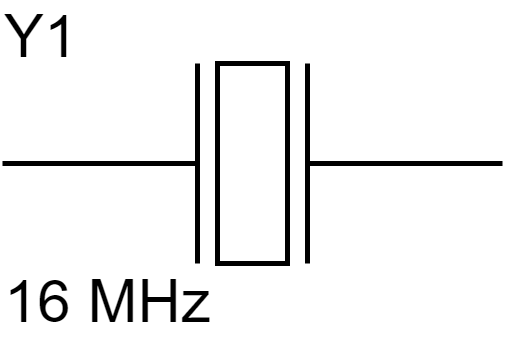
\includegraphics[height=1in]{electrical_schematics/oscillator_symbol.png}
            \caption[Oscillator Symbol]{Schematic symbol for crystal oscillators.}
        \end{figure}

        \subsubsection*{Switches}
        Switches are mechanical contacts that physically direct the flow of electricity.
        They can have multiple independent circuits called "poles" that can allow current to flow from a common connector to an output connector called a "throw".
        They are named according to their architecture, e.g. Single Pole Double Throw (SPDT) switches have one circuit with two outputs that are connected to the common pin, depending on the switch position.
        Double Pole Triple Throw (DP3T) switches have two circuits that connect three output pins to a common input pin, depending on the switch position.
        Each circuit is mechanically linked so the same output connector in both circuits will be connected to the common.
        One downside to the mechanical switch is that they can be welded together if a maximum current is exceeded or, they can wear out over thousands of cycles.

        % \begin{marginfigure}[-3in]
        %     \labfig{switch_real}
        %     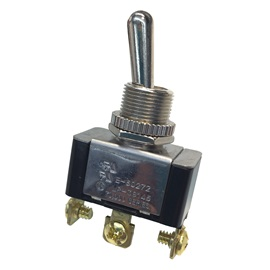
\includegraphics[]{electrical_schematics/switch.jpg}
        %     \caption{A common SPDT switch.
        %     Retrieved from \href{https://www.gardnerbender.com/en/p/GSW-12/SPDT-Toggle-Switch}{Gardner Bender}}
        % \end{marginfigure}

        \begin{figure}[h!]
            \labfig{switch_symbol}
            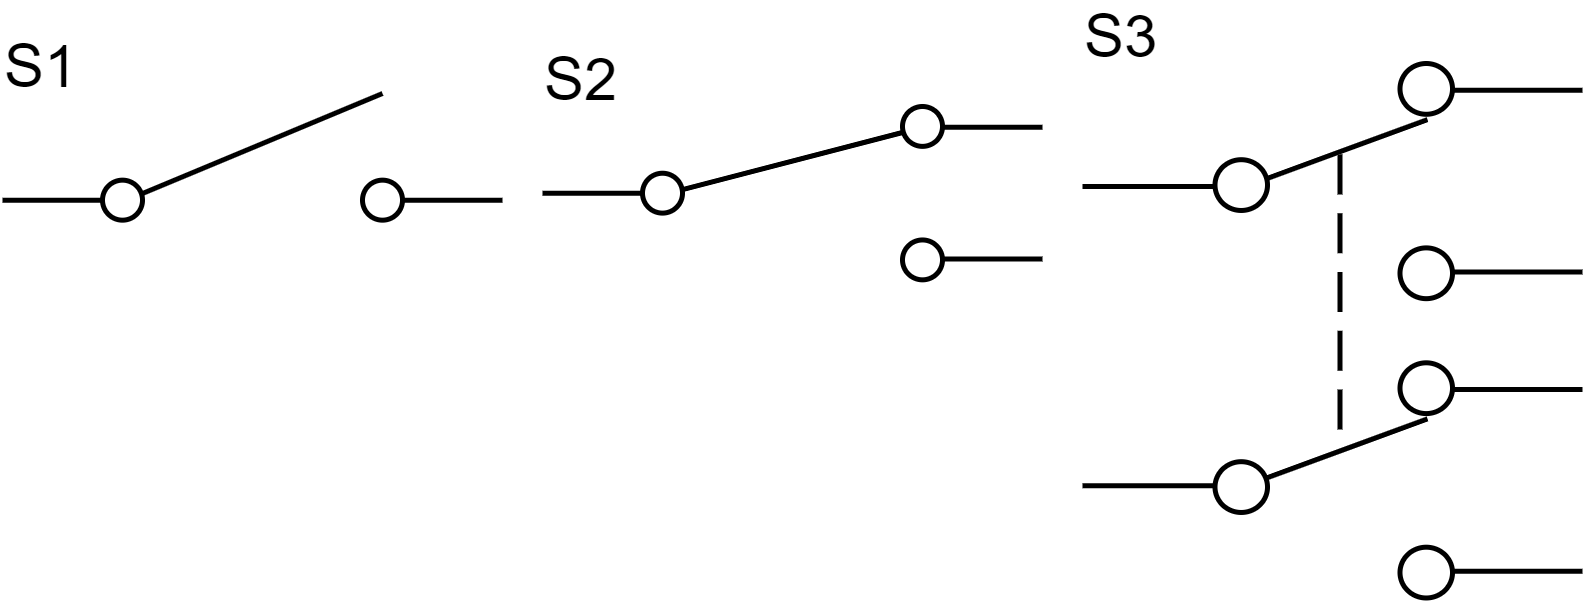
\includegraphics[height=1.5in]{electrical_schematics/switch_symbols.png}
            \caption[Switch Symbols]{Schematic symbols for different switch types.
            \emph{From left to right:} SPST, SPDT, DPDT.}
        \end{figure}

        \paragraph*{Buttons} are typically Single Pole Single Throw (SPST) switches that are spring loaded to remain normally open until pressed.
        When the button is pressed, a conducting plate makes contact with the common and output pins, completing the circuit through the button.
        These are commonly used as human input into circuits for calculations, state machines, typing lecture notes, etc.

        \begin{marginfigure}[-2in]
            \labfig{button_real}
            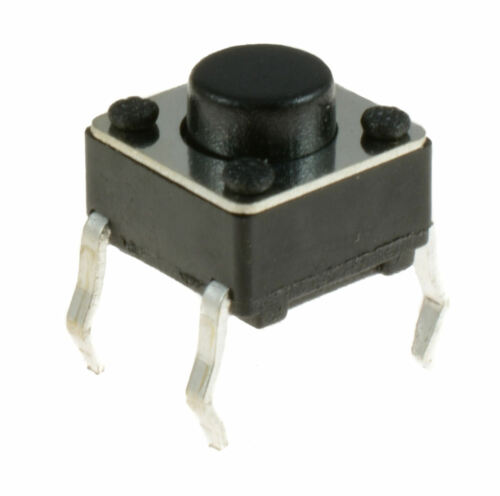
\includegraphics[]{electrical_schematics/button.jpg}
            \caption{A common push button found in most Arduino kits.
            Retrieved from \href{https://www.ebay.co.uk/itm/10-x-6x6x5mm-Momentary-Mini-Push-Button-Tactile-Switch-PCB-Mounted-SPST-/251779595483}{eBay}}
        \end{marginfigure}

        \begin{figure}[h!]
            \labfig{button_symbol}
            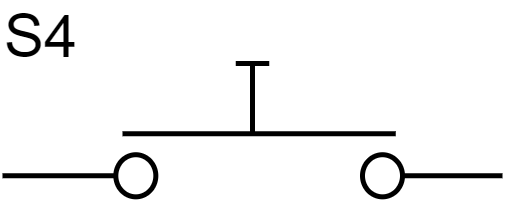
\includegraphics[height=0.75in]{electrical_schematics/button_symbol.png}
            \caption[Switch Symbols]{Schematic symbols for a normally open push button.}
        \end{figure}

        \paragraph*{Relays} are electromechanical switches that rely on an electromagnetic to move the electrical contact, rather than physical force.
        These are used for computers to manipulate large currents or direct electrical flow automatically, without human intervention.
        These relays follow the same nomenclature as normal switches and can be found in any number of configurations of poles and throws.

        \begin{figure}[h!]
            \labfig{relay_symbol}
            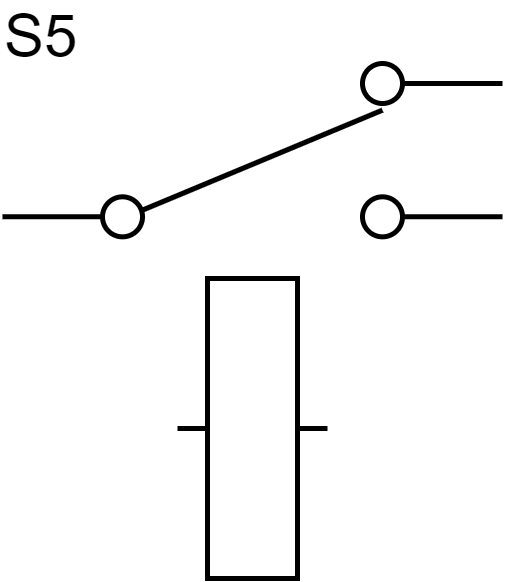
\includegraphics[height=1.5in]{electrical_schematics/relay_symbol.png}
            \caption[Switch Symbols]{Schematic symbols for an electromechanical relay.}
        \end{figure}

        \subsubsection*{Transistors}
        Transistors are electrical solid-state switches that use electrochemical properties to control the flow of electricity through them.
        These are typically able to withstand millions, if not billions, of switching cycles before failing and have driven the modern age we find ourselves in today.
        Everything in modern computing from the simple logic gate to the highest end computer and graphics processors use transistors to perform calculations or "think" about problems.
        Transistors have a gate that controls current flow from the source to the drain, depending on the voltage applied.

        \begin{marginfigure}[-1in]
            \labfig{transistor_real}
            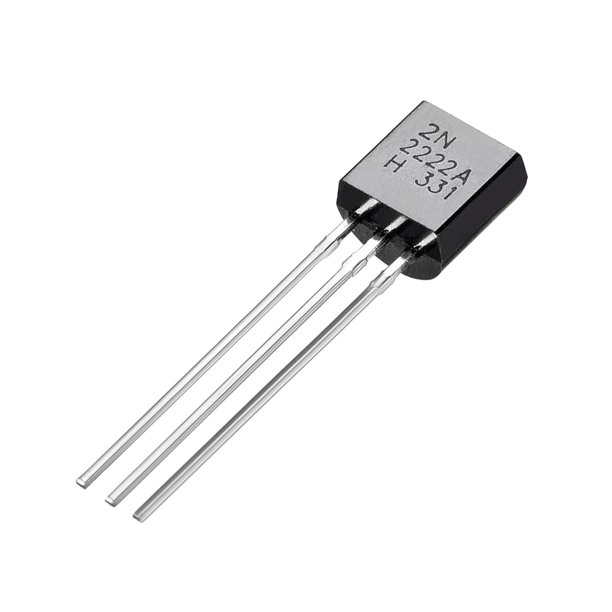
\includegraphics[]{electrical_schematics/transistor.jpeg}
            \caption{A common transistor found in most Arduino kits.
            Retrieved from \href{https://www.walmart.com/ip/2N2222A-Plastic-Encapsulate-Power-Transistor-NPN-TO-92-25PCS/283496991}{Walmart}}
        \end{marginfigure}

        \begin{figure}[h!]
            \labfig{transistor_symbol}
            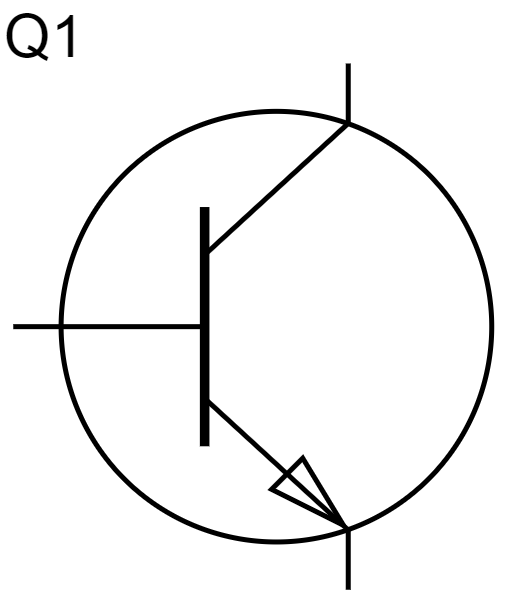
\includegraphics[height=1.5in]{electrical_schematics/transistor_symbol.png}
            \caption[Switch Symbols]{Schematic symbol for a transistor.}
        \end{figure}

        \paragraph*{MOSFETs} or Metal-Oxide-Semiconductor Field-Effect-Transistors are some of the most common types of transistors.
        They are able to be configured (doped) with different silicon structures that give them different electrochemical properties.
        N-Channel MOSFETs require a positive voltage on the Gate to function, whereas P-Channel MOSFETs require a negative gate voltage.
        Because of this, N-Channel MOSFETs are typically used for low-side switching (connect circuit to ground) and P-Channels are used for high switching (connect circuit to the voltage source). 
        There are two main types: depletion, which requires a Gate-Source voltage (Vgs) to switch the gate OFF, equivalent to a normally-closed switch; and enhancement where a Vgs is required to switch the gate ON, acting like a normally-open switch.
        These transistors are very common in high power applications and signal amplification.

        \begin{figure}[h!]
            \labfig{transistor_symbol}
            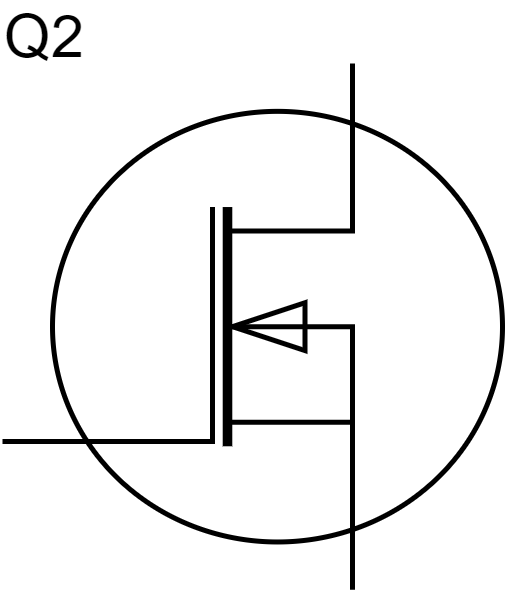
\includegraphics[height=1.5in]{electrical_schematics/pmosfet_symbol.png}
            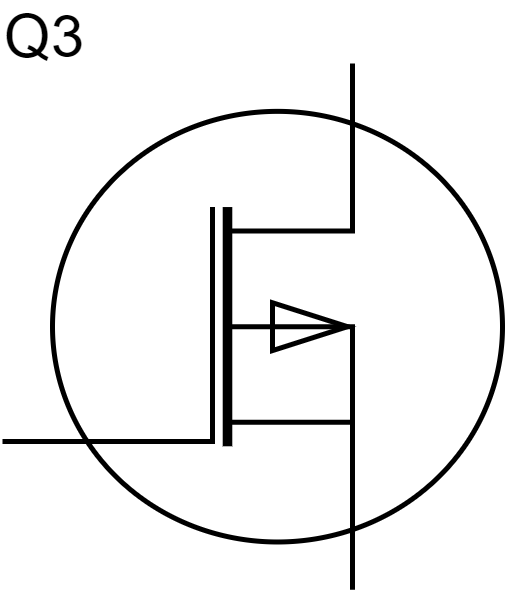
\includegraphics[height=1.5in]{electrical_schematics/nmosfet_synmbol.png}
            \caption[Switch Symbols]{Schematic symbols for MOSFETs.
            On the left is a P-Channel MOSFET, on the right is an N-Channel MOSFET.}
        \end{figure}

        \todo{insert example from Thetis/EVE circuits - cherry pick some nice ones that use mostly discreet components}

    \subsection{Integrated Circuits}
    Integrated Circuits (ICs) comprise the backbone of modern electrical design.
    They combine any combination of discreet components, logic gates, processors, storage, etc. into a single package that can be easily placed into a circuit.
    For schematic symbols, the representation varies wildly, but generally hold to a few core design features:
        \paragraph*{Outlines} - represents the chip's presence on the schematic. 
        It encompasses all of the information about the IC and usually is large enough to fit descriptive text and allows the pins to be arranged in a cohesive manner.

        \paragraph*{Pins} - schematic representations of the chip's physical contacts with the circuit. 
        Each is uniquely coupled to the physical pin or pad on the real-world design, but does not have to be sequentially ordered in the schematic.
        Each pin should have a label for its purpose on the IC next to it, within the outline, as well as a label to identify its physical number on the IC.

        \paragraph*{Name} - this is the unique identifier of the IC on the schematic

        \paragraph*{Values} - this is typically the IC's part number for ordering information and implementation

    It is important to note that some IC symbols will opt to include other handy information in the outline so it is more easily accessible without having to refer back to the datasheet constantly.

    \todo{insert image of an IC symbol with leaders pointed to different parts}

    \todo{Inlcude image of IC circuits e.g. voltage regulator}